
\subsection*{\textbf{Question 5.c)}}
\begin{quote}

\textbf{Problem}
\begin{quote}
Right now we want to improve this method, because NGP has several disadvantages. For this we are going to use a method which assumes that particles are cubes in 3D of uniform density and have the size of a grid cell. Calculatue how mass needs to be assigned in the case of this other method called the Cloud In Cell (CIC) method and implement it in code. To check the robustness of your implementation again make the same plots as before.
\end{quote}

\textbf{Solution} 
\begin{quote}
The mass needs to be assigned over the nearest 8 grid points. Each grid point gets thereby a fraction of the cube around the particle. The fraction assigned to a grid point here depends on the position of the particle and might be zero for some of the nearest 8 grid points. The way in which the mass is assigned to the nearest gird points is explained in the comment of the code that assigns the mass (page 73 ). The code that creates the plots and the plots them self can be found below.
\newpage
\end{quote}

\textbf{Code - Plots}
\begin{quote}
The code that creates the same plots as in 5.a and 5.b for a 3D grid with the CIC method.
\lstinputlisting[firstline = 74, lastline=122]{./Code/assigment_5.py}
\end{quote}

\newpage


\textbf{Plots - Slices}
\begin{quote}
\begin{figure}[!ht]
\centering
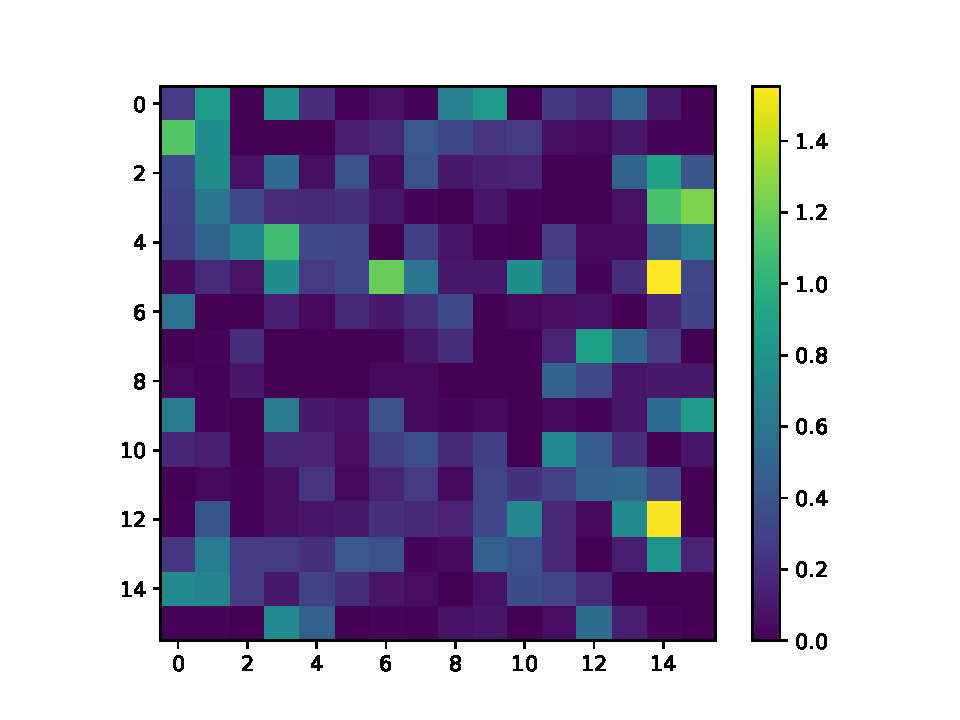
\includegraphics[width=14cm, height=9.5cm]{./Plots/5c_slice_4.pdf}
\caption{The x-y slice of the created mass grid with the CIC method for $z = 4$. The color indicates the assignment mass in terms of particle mass. Notice that the range of the colorbar deviates from the other three figures below.}
\end{figure}

\begin{figure}[!ht]
\centering
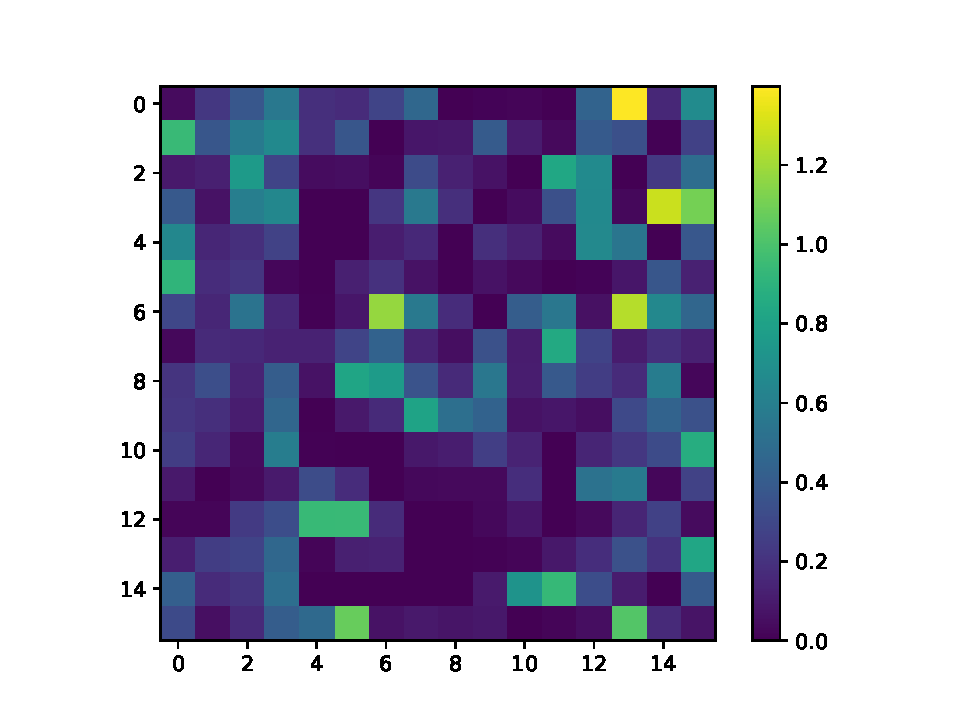
\includegraphics[width=14cm, height=9.5cm]{./Plots/5c_slice_9.pdf}
\caption{The x-y slice of the created mass grid with the CIC method for $z = 9$. The color indicates the assignment mass in terms of particle mass. Notice that the scalre of the colorbar deviates from the other three figures.}
\end{figure}

\newpage
\begin{figure}[!ht]
\centering
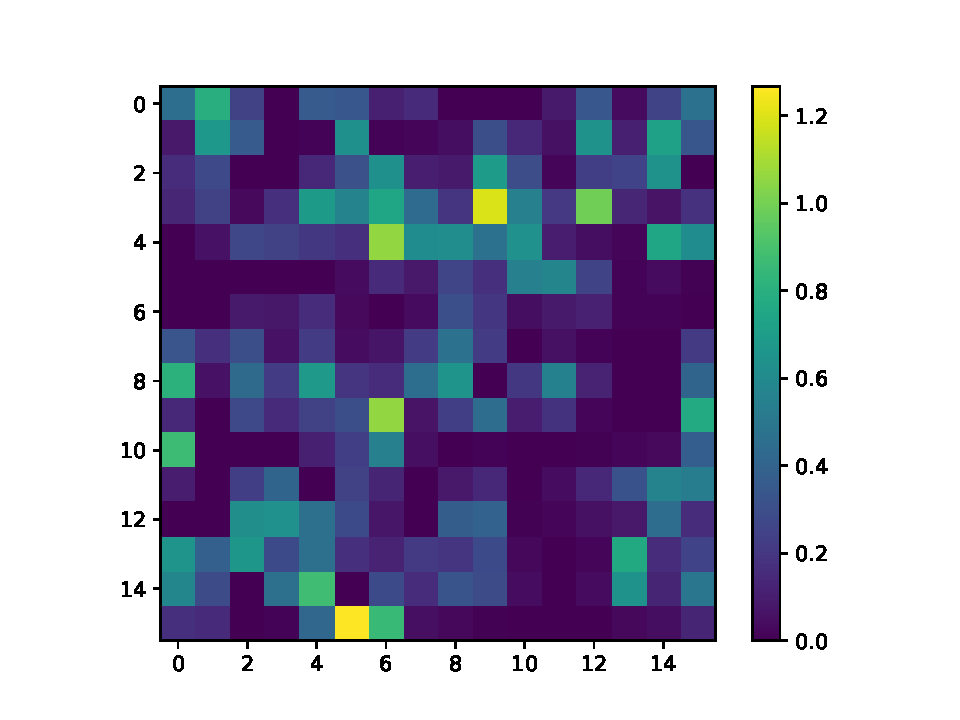
\includegraphics[width=14cm, height=9.5cm]{./Plots/5c_slice_11.pdf}
\caption{The x-y slice of the created mass grid with the CIC method for $z = 11$. The color indicates the assignment mass in terms of particle mass. Notice that the colorbar deviates from the other three figures. }
\end{figure}


\begin{figure}[!ht]
\centering
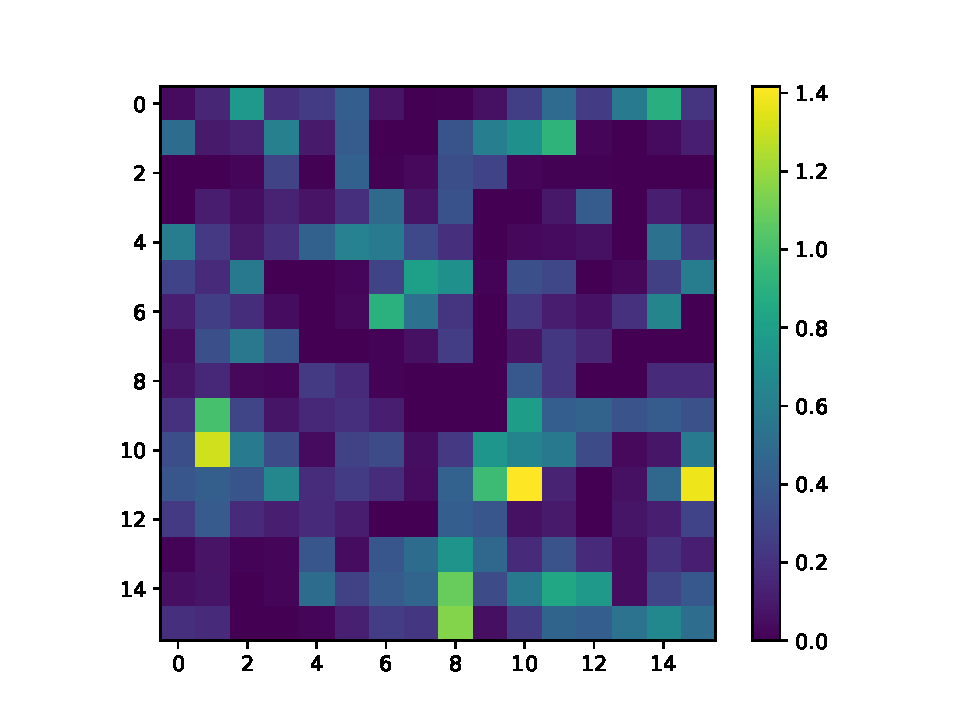
\includegraphics[width=14cm, height=9.5cm]{./Plots/5c_slice_14.pdf}
\caption{The x-y slice of the created mass grid with the CIC for $z = 14$. The color indicates the assignment mass in terms of particle mass.Notice that the scale of the colorbar deviates from the other three figures. }
\end{figure}
\newpage

\textbf{Plots - Cells}
\begin{quote}
\begin{figure}[!ht]
\centering
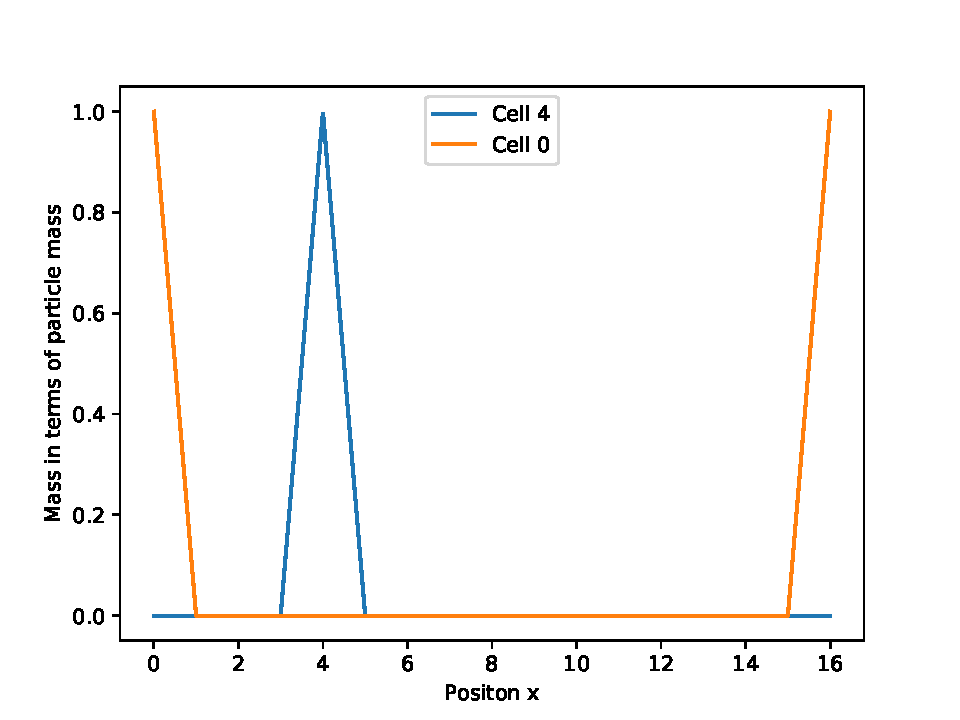
\includegraphics[width=14cm, height=9.5cm]{./Plots/5c_cell.pdf}
\caption{The mass assigned for a particle moving from x = 0 to x = 16 for the cloud in the cell method. The orange and red line respectively indicate the mass assigned to cells 0 and 4 as function of the position of the particle. The plot is created for a 3D  mass grid of size 16 with circular boundary conditions.  }
\end{figure}

\end{quote}
\end{quote}
\end{quote}











